\section{Results}
\label{sec:results}

% \begin{itemize}
%     \item Explain configs (same as PPO paper for MuJoCo)
%     \item Explain flow of runs (training, logging and evaluation processes)
%     \item Compare results with PPO paper (training plots [need to explain] and evaulation results)
%     \item Mention Streamlit app for render visualization.
% \end{itemize}

This section presents the performance of our PPO implementation across the selected environments. The training progress is illustrated with learning curves that show the average reward per step over each update cycle, and the final performance is compared with established benchmarks where applicable. All agents were trained for a specified number of timesteps, and their final performance was evaluated by averaging rewards over 100 test episodes generated with the learned policy, as detailed in the evaluation results CSV file (\texttt{results/evaluation\_results.csv}).

To further illustrate the learned behaviors, the trained agents can be visualized in action within their respective environments. For each environment, three pre-generated video renders showcasing the agent's policy are available in the `renders` subdirectory within the corresponding agent's results folder. Additionally, an interactive Streamlit application has been developed to facilitate this visualization. This application allows users to select an environment and generate new renders on-the-fly using our trained agents. The Streamlit visualizer can be accessed at: \url{https://ppo-visualizer.streamlit.app/}

\textit{Note:} When using the app, please mind that the render generation process may take several seconds to complete, especially for the MuJoCo environments, since it is being generated in real-time in the dedicated Streamlit Cloud machine.

\subsection{CartPole-v1}
The CartPole-v1 environment serves as a fundamental benchmark for reinforcement learning algorithms. The objective is to balance a pole on a cart for as long as possible. Our PPO agent was trained for 20,000 timesteps.

The agent successfully learned to solve this environment, achieving the maximum possible average reward of \textbf{500.0} over 100 test episodes. The learning curve, depicted in Figure~\ref{fig:cartpole_training}, shows a rapid increase in reward, quickly reaching and maintaining optimal performance.

\begin{figure}[H]
    \centering
    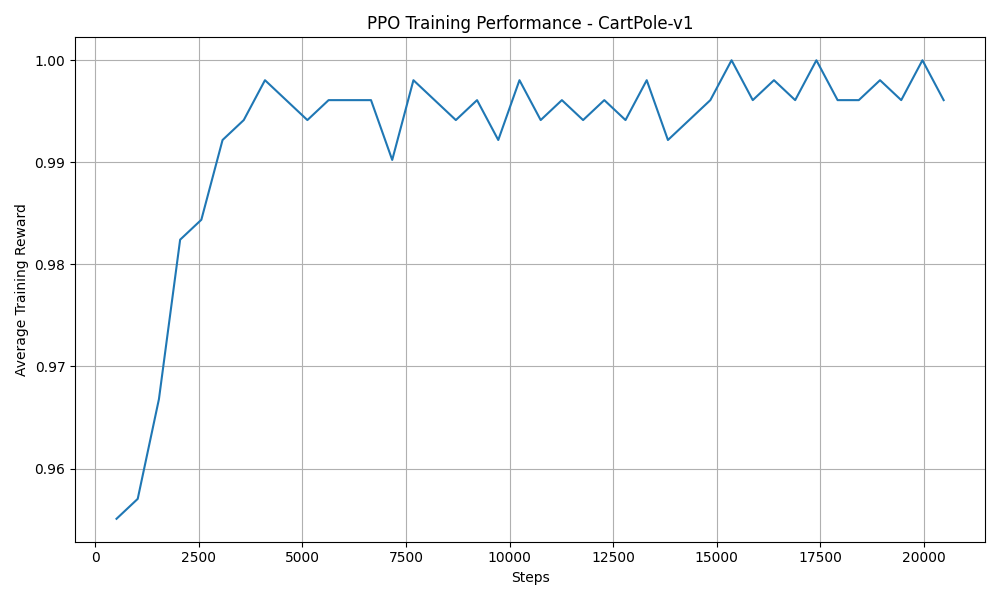
\includegraphics[width=0.8\textwidth]{figures/cartpole_training_plot.png}
    \caption{Training progress for PPO on CartPole-v1. The plot shows the average per-step reward (averaged over all steps taken during an update cycle) against training timesteps.}
    \label{fig:cartpole_training}
\end{figure}

This result confirms the fundamental correctness and effectiveness of our PPO implementation on a classic discrete control task. The configuration for this agent, detailed in the results CSV file. This is the only experiment for which we utilized shared features between the actor and critic and normalized advantages.

\subsection{HalfCheetah-v5}
HalfCheetah-v5 is a more complex continuous control task from the MuJoCo suite, where a 2D cheetah robot aims to run forward as quickly as possible. The agent was trained for 1 million timesteps.

Our PPO implementation achieved a final average reward of approximately \textbf{1770.62} over 100 test episodes. The training progress is shown in Figure~\ref{fig:halfcheetah_training}. The learning curve demonstrates steady improvement over the training duration, indicating successful learning in this high-dimensional continuous space, though with some variance typical of complex RL tasks.

\begin{figure}[H]
    \centering
    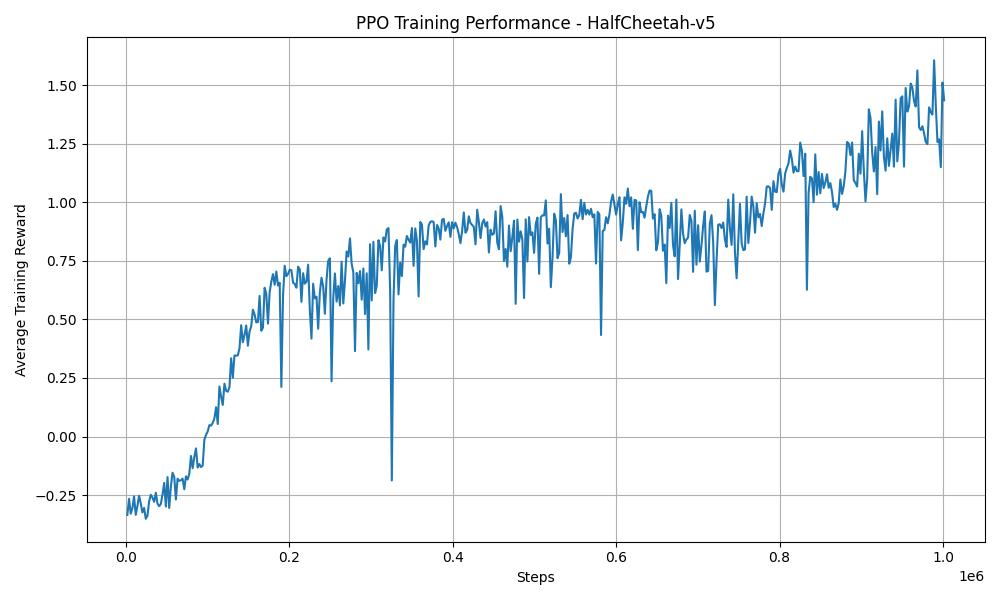
\includegraphics[width=0.8\textwidth]{figures/halfcheetah_training_plot.png}
    \caption{Training progress for PPO on HalfCheetah-v5.}
    \label{fig:halfcheetah_training}
\end{figure}

Comparing our result to the original PPO paper~\cite{schulman2017proximal}, which reports scores for PPO variants on HalfCheetah typically ranging from 1500 to 2100 after 1 million timesteps, our achieved score of approximately \textbf{1770.62} is well within this expected performance range. The configuration used for this experiment was based on the settings reported in the original PPO paper for MuJoCo environments, aiming to make our results as comparable as possible. Specific hyperparameter details can be found in the results file. Notably, this run employed separate networks for the actor and critic and did not normalize advantages.

\subsection{Reacher-v5}
Reacher-v5 is another MuJoCo continuous control task where a two-jointed robotic arm must reach a randomly positioned target. The agent was trained for 1 million timesteps.

The PPO agent achieved a final average reward of approximately \textbf{-8.45} over 100 test episodes. The learning curve is presented in Figure~\ref{fig:reacher_training}. The plot shows the agent quickly learning to improve its performance and stabilizing at an optimal policy.

\begin{figure}[H]
    \centering
    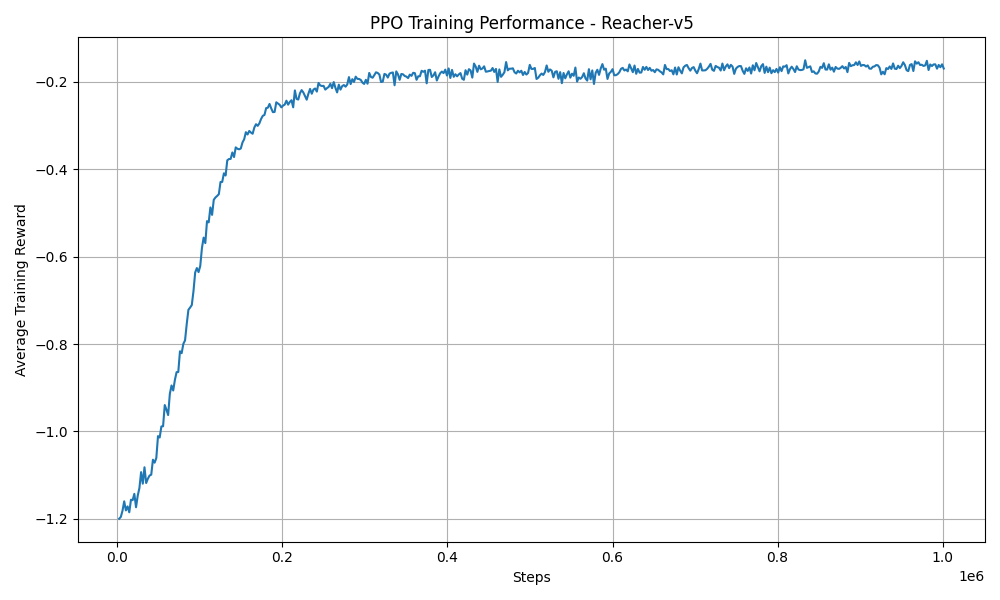
\includegraphics[width=0.8\textwidth]{figures/reacher_training_plot.png}
    \caption{Training progress for PPO on Reacher-v5.}
    \label{fig:reacher_training}
\end{figure}

The original PPO paper~\cite{schulman2017proximal} reports scores for Reacher typically around -5 to -10 after 1 million timesteps. Our achieved score of \textbf{-8.45} falls comfortably within this expected range, indicating a competent performance of our implementation on this task. Similarly to the HalfCheetah experiment, we used the same hyperparameters as in the original PPO paper for MuJoCo environments. The configuration details are available in the results file. This run also employed separate networks for the actor and critic and did not normalize advantages.

The results across these diverse environments demonstrate the capability of our PPO implementation to learn effective policies for both discrete and continuous control tasks, achieving performance comparable to established benchmarks.